
\documentclass[11pt]{iopart}
\usepackage[pdftex,bookmarks,pagebackref]{hyperref}

\usepackage{epsfig}
\usepackage{color}

\usepackage{amssymb}
\usepackage{amsfonts}
\usepackage{graphicx}
\usepackage{iopams}
\graphicspath{figures/}
\usepackage{lineno}

\newcommand{\dsnote}[1]{{\color{green}[#1]}}
\newcommand{\sjnote}[1]{{\color{red}[#1]}}

%%%%%%%%%%%%%%%%%%%%%%%%%%%%%%%%%%%%%%%%%%%%%%%%%%%%%%%%%%%%%%%%%%%%%%%%%%%%%%%%%%%%%%
\begin{document}

\title[Gate Hadron PET]{GATE simulation of hadrontherapy treatment
  combined with a complete PET imaging system for dose monitoring : a
  feasibility study}

%Feasibility of a Monte Carlo full-scaled
%  simulation of patient dose deposition combined with PET imaging
%  during pencil beam spot scanning with $^{12}$C ion beams using GATE
%  on a HPC cluster}

\author{S{\'e}bastien Jan$^{1}$, Thibault Frisson$^{2,3}$, and David Sarrut $^{2,3}$}

\address{$^1$ CEA, Service Hospitalier Fr{\'e}d{\'e}ric Joliot, Orsay, France}
\address{$^2$ University of Lyon, CREATIS; CNRS UMR5220; INSA-Lyon, France}
\address{$^3$ University of Lyon, L\'eon B\'erard Cancer Center, F-69373, Lyon, France}
\ead{sebastien.jan@cea.fr}
%david.sarrut@creatis.insa-lyon.fr}

%%%%%%%%%%%%%%%%%%%%%%%%%%%%%%%%%%%%%%%%%%%%%%%%%%%%%%%%%%%%%%%%%%%%%%%%%%%%%%%%%%%%%%
\linenumbers
\begin{abstract}

  {\it

    We used GATE to perform Monte-Carlo simulations of a hadrontherapy
    cancer treatment combined with the complete description of a PET
    imaging device for dose monitoring. Dose distribution and PET
    images were obtained from a carbon ion beam irradiation using
    pencil beam spot scanning delivery. We study the produced data
    to analyse the interest of using a full PET system simulation
    instead of usual Gaussian smoothing. 

    This study shows the possibility to simulate with the same
    Monte-Carlo platform a complex scanning treatment and the
    associated imaging system. We also show that it scales well on a
    large number of CPUs. Differences in the distal position of the
    signal falloff of 18\% between full TEP system simulation and
    Gaussian model were found.  To our knowledge, it is the first
    full-scale simulation in the context of hadrontherapy including
    dose monitoring with PET imaging with the same simulation
    framework. We believe that the GATE plateform is well suited to
    perform highly realistic simulations in the field of
    hadrontherapy, combining dose and imaging system to monitor the
    dose delivery during a cancer treatment. This approach could be
    use to develop and optimize imaging devices and to determine the
    feasibility of quantitative imaging protocols.
    
    % The dose monitoring for $^{12}$C irradiation should be
    % realistic and feasible for a target dose higher than 1 Gy.
    % Methods.Using the GATE platform; explicit simulation from the
    % beam to the patient and from the patient to the PET scanner
    % system. Scaling was assessed on a 1000 CPUs cluster.
  }

  
\end{abstract}

%Uncomment for PACS numbers title message
%\pacs{00.00, 20.00, 42.10}
% Keywords required only for MST, PB, PMB, PM, JOA, JOB? 
\vspace{2pc}
\noindent{\it Keywords}: Monte Carlo ; GATE ; Hadrontherapy ; PET monitoring
% Uncomment for Submitted to journal title message
%\submitto{\PMB}
% Comment out if separate title page not required
\maketitle


%%%%%%%%%%%%%%%%%%%%%%%%%%%%%%%%%%%%%%%%%%%%%%%%%%%%%%%%%%%%%%%%%%%%%%%%%%%%%%%%%%%%%%%
\section{Introduction}

Monte Carlo simulations are essential for many medical applications,
especially for imaging and radiotherapy. Numerical approaches for
imaging applications are used to design new devices, to optimize and
study the effect of different acquisition parameters on the image
quality. They are also extremely useful to validate and assess
compensation methods and image reconstruction techniques. In radiation
therapy, Monte Carlo simulations are used to develop fast dose
deposition algorithms or to characterize beams properties. The
GATE~\cite{Jan2004, Jan2011} open-source simulation platform, based on
the Geant4 toolkit~\cite{Allison2006, Agostinelli2003}, has been
developed and used since 2002 by the OpenGATE collaboration.  The work
presented here consider Positron Emission Tomography (PET) as a method
for in situ monitoring of carbon hadrontherapy. This method considers
the image of the radioactivity distribution induced by the nuclear
fragmentation processes occurring during the
irradiation~\cite{Enghardt1999}. Such distribution has been shown to
be correlated with the dose distribution~\cite{Moteabbed2011}, leading
to interesting perspectives in dose monitoring, even if exact
quantification is still studied (e.g. the biological washout effects
due to blood perfusion and metabolism, deteriorates this
correlation~\cite{Parodi2008}).

In this scope, we propose to illustrate the usability of GATE as a
tool to study the relationship between the PET image quality and the
deposited dose. To our knowledge, GATE is the only Monte-Carlo
platform allowing to simulate in the same framework all the range of
physical events occurring during such a hadron-PET scan. As example,
it has been successfully used in PET imaging~\cite{Buvat2006a} and for
hadrontherapy dose simulations~\cite{Jan2011, Grevillot2011a}. We
defined a realistic simulation setup that includes a model of a
realistic $^{12}$C pencil beam scanning, a numerical patient based on
a thoracic CT scan and a PET camera model for the image acquisition
system. This study aims to provide a proof of concept about GATE used
to produce hyper-realistic simulations to estimate the PET efficiency
for therapeutic control in the case of hadrontherapy treatments, to
optimize the design of dedicated PET detectors and to identify the
best protocols to control and follow the deposited dose. These
simulations were performed on a supercomputer (Computing Center for
Research and Technology) using around 1000 CPUs to demonstrate the
high scalability of the platform.


% First results of GATE simulations including a carbon ions ($^{12}$C)
% irradiation of a lung tumour followed by a full PET acquisition are
% presented. 

%%%%%%%%%%%%%%%%%%%%%%%%%%%%%%%%%%%%%%%%%%%%%%%%%%%%%%%%%%%%%%%%%%%%%%%%%%%%%%%%%%%%%%%
\section{Method}

% \cite{Sommerer2009}

% \cite{Sommerer2006,Pshenichnov2007,Ponisch2004,Parodi2008,
%   Parodi2007,Parodi2002,Parodi2000,Parodi2007a,Hishikawa2002,
%   Fiedler2008,Crespo2006,Enghardt1999,Attanasi2009,Pshenichnov2006}

\subsection{Two steps approach}

We considered the simulation in two parts. The first part simulated
from the $^{12}$C beam at the exit of the nozzle to the
patient. Variables (energy, dose, position) were stored for primary
and secondary particles and specially $\beta^+$ emitters distributions
created during nuclear processes. At this level, we used a phase space
approach and the spatial distributions of $\beta^+$ emitters were
stored. These 3D maps were used as an input files for the PET scan
acquisition which were the second part of the simulation. This two
steps approach was design to give users opportunities to test
different configurations for the imaging system with the same
deposited dose distribution. With this strategy, it is also possible
to model in-beam prompt-gamma dose monitoring
strategy~\cite{Testa2008, Moteabbed2011} if information regarding the
gamma prompts produced by $^{12}$C nuclear reactions during tissue
interactions, are stored in dedicated files.  This approach does not
induce a penalty regarding the total computing time of the simulation.

% This gamma prompts file should be also used as a phase space for
% imaging modeling.  When created, such emitters were stopped during
% the simulation and

\subsection{Simulation setup: target and beam delivery}

\subsubsection{CT Target}

The geometry of the simulation setup is as follows. Target was
imported from a X-Ray Computed Tomograph (CT) image resampled to
isotropic $2^3$ mm$^3$ voxel size (1.7 million voxels). Image was
described with the method proposed in~\cite{Sarrut2008} allowing fast
particle navigation through the matrix of voxels. Hounsfield units
where converted into Geant4 materials thanks to the stoichiometric
calibration method proposed in~\cite{Schneider2000a}. A density
tolerance of $0.1 g/cm^3$ was used leading to $30$ different Geant4
materials, with atomic composition interpolated from 7 initial
materials (Air, Lung, Adipose Tissue, Adrenal Gland, Soft Tissues,
Connective Tissue, Marrow Bone) according to the mass density. The
numerical phantom used for this study is a public patient image of a
4D CT thoracic acquisition~\cite{Vandemeulebroucke2007} including a
lung tumour on which an approximated gross tumour volume (GTV) was
manually delineated.

\begin{figure}[!h]
\centering
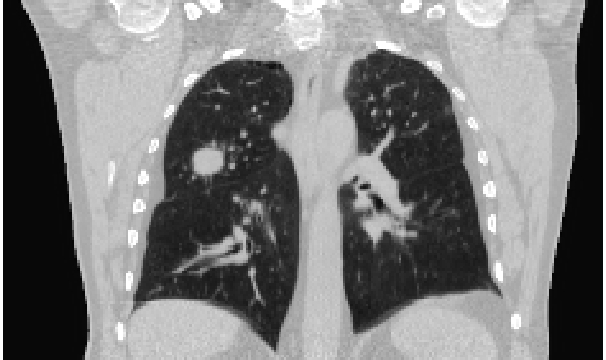
\includegraphics[width=6cm,height=40mm]{figures/phantomCT.jpg}
\caption{Coronal slice of the thorax CT used for this study. Tumour
  target is clearly visible in the center of the parenchyma on the
  right lung (left of the image).}
\label{fig00}
\end{figure}

\subsubsection{Physics list}

As recommended by the Geant4 Electromagnetic (EM) Standard working
group for medical physics applications~\cite{G4EMGroup2010}, we used
the (EM) standard package with the option 3 (Opt3) list of
parameters. Regarding hadronic interactions, we followed the
recommendation of~\cite{Pshenichnov2007, Zacharatou2008}. One
difference was, following~\cite{Polf2009, Peterson2009,
  Grevillot2010}, that we used the precompound model as inelastic
hadronic model even above 80 MeV, unlike in~\cite{Pshenichnov2007},
that have been found to be closer to measurement in proton
experiments. Very recently, Bohlen et al~\cite{Bohlen2010} proposed an
interesting study comparing nuclear fragmentation models of FLUKA and
Geant4 for carbon ion therapy, and gave indication to better tune
Geant4. Those recommendation will be included in future works.  In the
case of this study, we are focused on the positron emitter production
($^{11}$C and $^{15}$O) for dosimetry monitoring by PET imaging. As it
was shown by Pshenichnov et al.~\cite{Pshenichnov2006}, the numerical
model overestimates the cross section production for $^{11}$C and
$^{15}$O of 15\% to 20\% according to
measurement~\cite{Parodi2007a}. This will be directly correlated to
the PET signal with an overestimation in the same range.

% \begin{table}[htbp]
% \begin{center}
%   \begin{tabular}{|c|c|c|c|c|c|c|} \hline
%     $^{12}$C energy  & \multicolumn{2}{|c|}{212.12 A MeV}  & \multicolumn{2}{|c|}{259.5 A MeV}  & \multicolumn{2}{|c|}{343.46 A MeV}       \\
%     \cline{2-7} & Simulation & Experiment & Simulation & Experiment &
%     Simulation & Experiment \\ \hline \hline 
%     $^{11}$C             & 11.9  &  10.5  &  16.8  &  14.7  &  25.25  &  19.9      \\ \hline
%     $^{15}$O             & 2.38  &  2.1  &  3.69  &  3.1   &  6.09   &  5.0        \\ \hline \hline 

% \end{tabular}
% \end{center} 
% \caption{\it Production yields of positron emitter nuclei (per beam particles in \%) in a PMMA phantom: Geant4/GATE simulation versus experimental data.} 
% \label{tab:CrossSection}
% \end{table}

% \dsnote{D'ou tiens tu ces valeurs ? Tes manips ? S'il c'est deja publie dans un papier, pas la peine de le remttre me semble t il.}\\
% \sjnote{Valeurs deja publiees par Pshenichnov sur la base de mesure faites au GSI par Parodi mais c est un point fondamental donc je pense que c est bon pour le lecteur d'avoir concretement les valeurs sous les yeux et de ne pas avoir a revenir sur un article precedent. C est quand meme un point clef ou tu vois clairement l'overestimation de la simulation sur la production d emetteurs de positons et ca va donc artificiallement dans le sens d'une amelioration de la qualite d'image PET au final.}

\subsubsection{Scanned beam delivery system}

We considered a virtual beam delivery system inspired from the one
described in~\cite{Kramer2000a}. Scanning is achieved with
superimposition of multiple carbon ion spots varying in lateral and
longitudinal directions, and in energy. The scanning is intended to
spread out the dose such that the target volume receive an uniform and
high dose.  Given a beam direction, the distal plane of the target
volume was sampled with spots positions every 1.5 mm. Each spot was
mono-energetic, have a symmetric Gaussian profile of 5 mm FWHM and was
directed towards its end point in the distal plane. We considered
energy layers every 2 mm (about 3 MeV). We defined a simple pencil
beam model following~\cite{Grevillot2010}. We considered a unique spot
size, even if generally, the size depends on the beam energy. More
advanced descriptions of a pencil beam scanning delivery technique can
be performed~\cite{Grevillot2011} when focus on a real facility. In
Carbon facilities, such as at HIT or GSI, the irradiation delivered by
the synchrotron is pulsed, with spills (beam extraction) during few
seconds (max 2 s) and spill period of about 5s, required for beam
injection and acceleration. We considered here a continuous time
structure and did not split it into spills. We did not also consider
the time required to switch energy between two iso-energy slices,
which is typically in the range of 1-2 s~\cite{Rietzel2010}. The
optimization of each spot intensity was performed according to the
simplified one-dimensional method of~\cite{Kramer2000a} in order to
obtain uniform dose in the target part. Optimization was performed
field by field (single field uniform dose, SFUD~\cite{Lomax1999}). We
used a precomputed database of depth deposited energy profiles in
water. The database contained profiles with energy from 160 MeV/u to
230 MeV/u, with a 0.05 mm depth resolution and was computed with
multiple GATE simulations and stored in a database. Water Equivalent
Path Length (WEPL) were computed for all lines going from the virtual
beam source to each spot positions in the distal plane and
intersecting the CT voxels. Total WEPL was estimated by summing the
individual WEPL along all intersected voxels weighted by the
intersection length. WEPL for a given material was computed with an
approximation of the relative stopping power (to water) computed with
the Bethe-Bloch formula: $wepl = \rho \frac{Z/A}{0.555}$, with Z and A
the atomic and $\rho$ the mass density of the material.

We considered 3 fields leading to approximately 6000 individual
spots. It does not correspond to real treatment plans but aims at
describing representative test case. Typical irradiation dose-rate is
5 GyE/min/l~\cite{Noda2007}, corresponding to an intensity of
$1.2\times 10^9$ pps (particles per seconds). Regarding the proposed
pencil beam description, we thus considered that $10^8$ to $10^9$
particles reaching the patient correspond to 1 Gy to 10 Gy in the
tumour. We consider five different configurations, described later in
table~\ref{tab:setup}.


%dose relat / absolue ; no RBE (?) mentionner LET is available in each voxel
%=> chercher dose max par fraction (pas en GyE)
%cf url send to Seb

%http://totlxl.to.infn.it/mediawiki/index.php?title=Water_equivalent_path_length
% **IMAGE OF ALL BP**
% dsarrut@oronge:~/src/tinytps/BeamLines/RBE1
%% ~/src/tinytps/Simulations/Test2

%~/recherche/grandChallenge/simulations/lung/mac_patient2_3> 
% grep "/gps/source/add" spots1-lung.mac | wc -l 1973
% grep "/gps/source/add" spots2-lung.mac | wc -l 1937
% grep "/gps/source/add" spots3-lung.mac | wc -l 2034

% The two beam descriptions (beam1.mac and beam2.mac) used into
% main.mac, correspond to the physical dose SOBP optimization. The file
% beamRBE.mac corresponds to the results of a SOBP optimization perform
% with a single field on biological dose computed with [Kase2006]
% method.

\subsubsection{Scorers}

Dose was scored with the GateDoseActor described
in~\cite{Jan2011,Sarrut2008} that stores deposit dose and energy
distribution in a 3D matrix of dosels, together with the associated
statistical uncertainty. We choose a matrix of dosels of size $2^3
mm^3$.  We also stored the 3D distribution of points of creation of
$\beta^+$ emitters during the irradiation. We limited emitters scoring
to the two main ones, $^{11}C$ and $^{15}O$~\cite{Pshenichnov2007},
the others ($^{10}C$, $^{13}N$, $^{14}O$, $^{17,18}F$, $^{30}P$, for
those with more than 10s of half-live) were considering to have
negligible influence on a reconstructed PET image but could also be
stored if needed. The energy deposited by secondary particles and
specially by $\beta^+$ emitters in this case, was taking into account
in the dose and energy 3D matrices.

%\textbf{SEB : est ce que la dose (faible?) d{\'e}pos{\'e}e par ces emitters est prise
%en compte ? A indiquer ici} YES.

%to compare to [attanasi 2009] (events collected during 6 times 10 Gy.)

\subsection{PET scan for dose monitoring}

The conventional approach to model the PET acquisition in the case of
dose monitoring for hadrontherapy applications, is to convolve the
$\beta^{+}$ emitter map with a Gaussian function which is determined
by the point spread function (PSF) of the PET
system~\cite{Parodi2007a}. With this simplified method, the scanner
sensitivity is not taken into account. We think that it could be a
critical point for evaluating the relation between the deposited dose
and final PET image. For this reason, we propose a full Monte Carlo
simulation of the PET system. The system is the commercial ECAT EXACT
HR+~\cite{Brix1997} PET by Siemens. It is made of four rings of BGO
blocks partially cut into an 8x8 array of crystals measuring
4.0x4.1x30 mm$^3$ each, resulting in a 82.7cm diameter detector
cylinder and an axial field-of-view (FOV) length of 15.5cm. We defined
the BGO blocks, a back compartment to simulate the back scattering
induced by the light collection system, the lead end-shielding, and
the patient bed. The simulation assumes an energy resolution for each
crystal randomly drawn from a uniform distribution varying between $20
\%$ and $30 \%$ at 511 keV. The determination of the hit crystal is
based on the crystal with the highest energy deposition, to which an
additional analytical spatial blurring based on a 2D Gauss kernel can
be applied to model the decrease induced by the tube photomultipliers
of the Anger camera. A global sensitivity factor is also defined for
each block to replicate the sensitivity performance of the scanner;
this efficiency factor is set at $90 \%$ in the case of the HR+. This
PET scanner was already modelled and validated by using GATE and all
results are described in~\cite{Jan2005}. It is important to note that
it is not an in-beam PET configuration and we do not consider prompt
gamma and neutron contamination during the acquisition.

% This is the reason which
% explain that gamma prompt and neutron productions are note taken into
% account in our physical processes.

% Figure~\ref{fig:fig0} illustrates
% the global geometry of the HR+ scanner. 
% \begin{figure}[!h]
% \centering
% 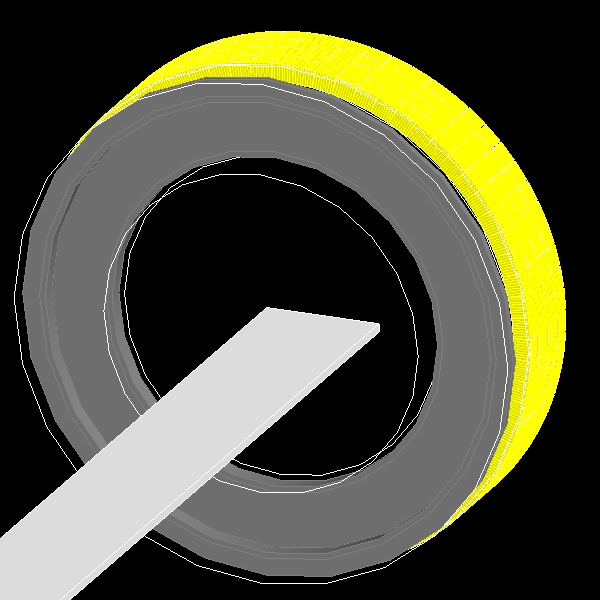
\includegraphics[width=40mm,height=40mm]{figures/HR_Simu_Gate_GC.jpg}
% 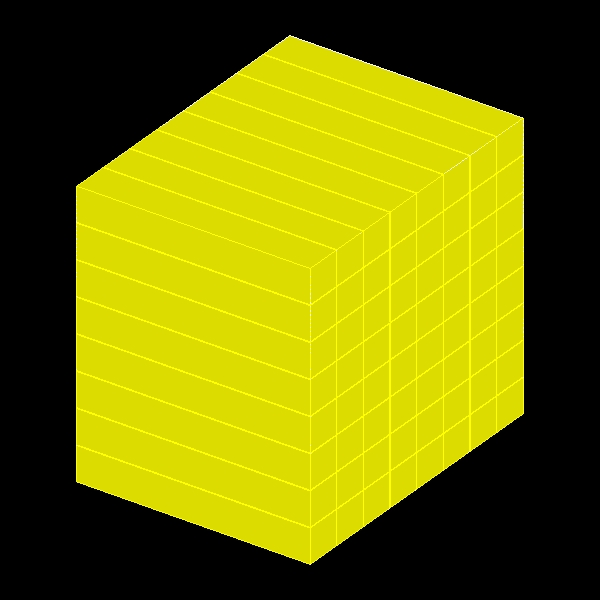
\includegraphics[width=40mm,height=40mm]{figures/bloc_detec_HR.jpg}
% \caption{Illustration of the HR+ PET scanner simulated with GATE
%   (Left). At right, one of the 288 blocks PET detectors which is
%   composed by 64 BGO crystals. \dsnote{C'est pas très beau ... (si je
%     peux me permettre). Allez, un effort, tu peux faire un truc qui
%     pete non ? }\sjnote{Je sais mais il faudrait installer une visu genre VRML pour G4 et faire re-tourner les géometries....ca me fait un peu chi...tu penses que c est indispensable ? Je pourrai aussi virer l'illustration mais je me dis que pour la communauté hadron, c est enfonce le clou sur le fait qu on modelise explicitement le systeme d'imagerie.}}
% \label{fig:fig0}
% \end{figure}

\subsubsection{PET acquisition and image reconstruction}

The energy window was set to 350-650 keV and the coincidence time
window to 12ns. The PET acquisition was started just after the
irradiation. The acquisition time was 10 minutes.  To improve the
image quantification, the simulated data were normalized, attenuated
corrected and reconstructed using the 3D OSEM
method~\cite{OSEM_ref}. We used the PET analytic simulator,
ASIM~\cite{Comtat1999} to produce the normalized sinogram. For the
attenuation correction, coefficient factors (ACFs) were also
calculated with ASIM using the voxelized attenuation map description
provided by the numerical patient phantom. \dsnote{Peux tu ajouter une
  conclusion en 1 phrase de cette partie, en argumentant sur le fait
  que cette simu est raisonnablement réaliste et en indiquant les
  limites ou améliorations éventuelles ? + REFS BIBLIO}

\subsection{Running GATE on a High Performance Computing machine}

All the simulations were running at the French Rechearch and
Technology Computing Center~\cite{CCRT} on the TITANE
supercomputer. This is a cluster integrating 1596 Bull NovaScale R422
servers, with 2 Intel Xeon 5570 quad core processors each including a
memory of 3 Go per core. With 3192 Intel Xeon 5570 4 cores, TITANE
offers a processing capacity above 90 teraflops, and 25 terabytes of
core memory, which put it in june 2009 in 38th place of the worldwide
supercomputer sites Top500 ranking. The TITANE cluster operates the
Bull HPC software platform that includes the Linux operating system
and the global and parallel Lustre file system. This platform is based
on an open source software integrated and optimized by Bull's HPC
competence center in Echirolles, France. GATE simulations were split
into similar jobs having different random seeds. Tools are in
developments to allow simplified access to this kind of computing
resources~\cite{Camarasu-Pop2010}.  For imaging part, jobs are
splitting following the PET acquisition time and including the
positron emitters decay time.

\subsection{Quantitative analysis}

For quantitative analysis of PET images, we consider the distance $L$
between the 50\% distal falloff (DFO) and the peak position as
illustrated on the figure~\ref{fig:dfo}. We first considered three
configurations corresponding to three dose values delivered to the
tumour : 1, 5 and 10 Gy ($S_{1}$, $S_{2}$, $S_{3}$). An additional
configuration $S_{1}^{*}$ was performed with Gaussian smoothing to be
compared to full PET system simulation ($S_{1}$). The configuration
$S_{3}^{*}$ was performed to evaluate the interest to consider
$^{15}O$ isotope in addition to $^{11}C$. Finally, to quantify the
influence of the dose on the image quality, we compared the
configurations $S_{3}$, $S_{2}$ and $S_{1}$. The table~\ref{tab:setup}
describes the parameters of the five studied configurations.

\begin{figure}[!h]
  \centering
  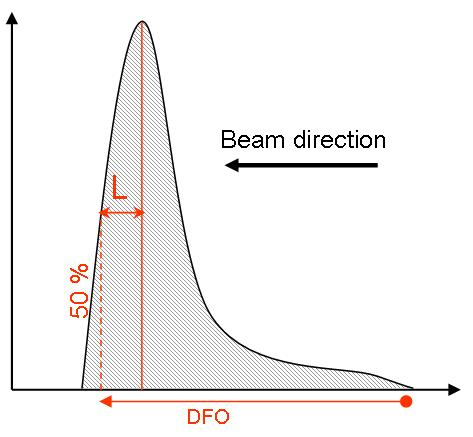
\includegraphics[width=65mm,height=45mm]{figures/dfo.jpg}
  \caption{$L$ parameter estimation to define a quantitative estimator
    in this study.\dsnote{Ajoute les unités aux axes. Peux tu faire
      venir le beam de la gauche (je préfère la gauche)}}
\label{fig:dfo}
\end{figure}

 
\begin{table}[htbp]
  \begin{center}
    \begin{tabular}{|c|c|c|c|c|} \hline
      Simulation   & $^{12}$C number  & Dose to   & PET simulation  & $\beta^{+}$ emitter  \\
      configuration               &                &  tumor (Gy)  & mode & contribution \\\hline \hline
      
      $S_{1}$    & $3.10^{8}$             & 1                     & Full GATE           &           $^{11}$C      \\ \hline
      $S_{1}^{*}$    & $3.10^{8}$         & 1                     & Gaussian Smoothing  &      $^{11}$C           \\ \hline
      $S_{2}$    & $15.10^{8}$            & 5                     & Full GATE           &       $^{11}$C          \\ \hline
      $S_{3}$    & $3.10^{9}$             & 10                    & Full GATE           &           $^{11}$C      \\ \hline
      $S_{3}^{*}$ & $3.10^{9}$            & 10                    & Full GATE           &  $^{11}$C + $^{15}$O    \\ \hline \hline 
    \end{tabular}
  \end{center} 
  \caption{\it Setup description: Carbon ions beam, target dose and PET simulation approach.}
  \label{tab:setup}
\end{table}

%%%%%%%%%%%%%%%%%%%%%%%%%%%%%%%%%%%%%%%%%%%%%%%%%%%%%%
\section{Results and discussion}

The figure~\ref{fig:fig1} illustrates the dose deposited during the
irradiation and the $\beta^+$ emitter maps for $^{11}$C and $^{15}$O
isotopes which are produced by $^{12}$C interactions for the setup
$S_{3}$. These images represents a qualitative proof of concept of the
GATE capabilities to perform complete and realistic simulations in the
field of hadrontherapy coupled with a nuclear imaging device.

\begin{figure}[!h]
  \centering
  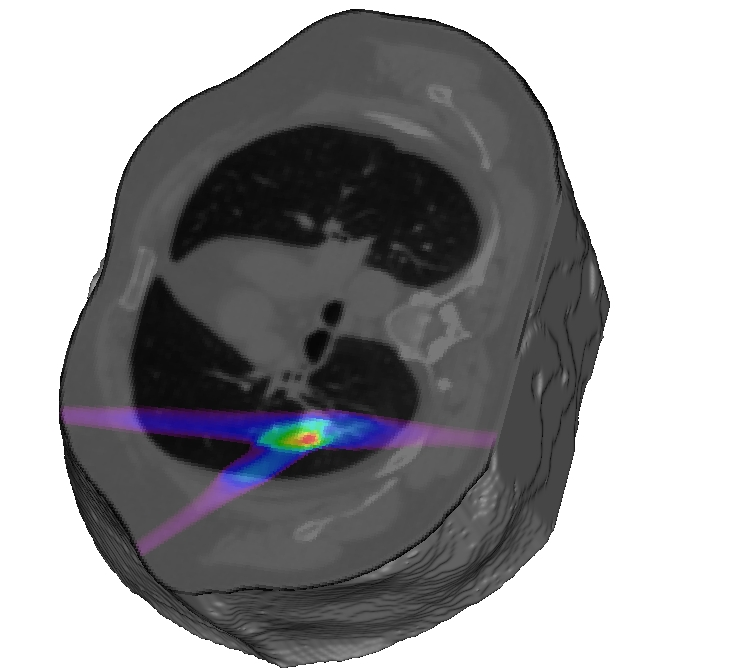
\includegraphics[width=55mm,height=35mm]{figures/3D-Dose_poumon.jpg}\\
  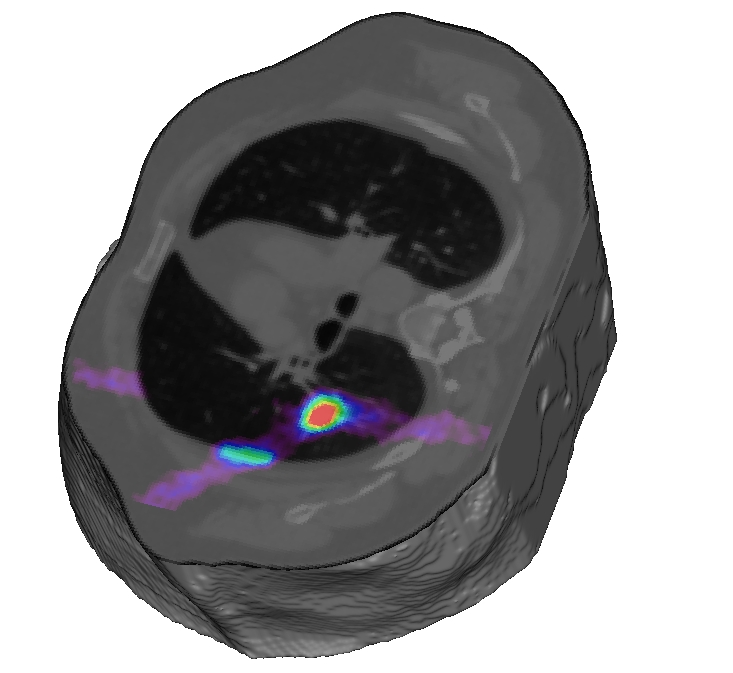
\includegraphics[width=55mm,height=35mm]{figures/3D-PETC11_poumon.jpg}
  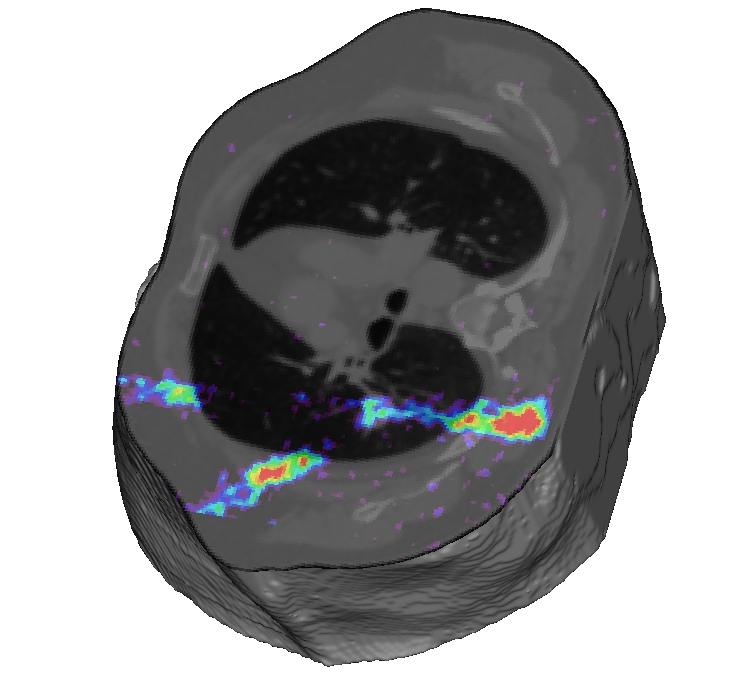
\includegraphics[width=55mm,height=35mm]{figures/3D-PETO15_poumon.jpg}
  \caption{Top : deposited dose distribution. Bottom-left: PET image
    considering only $^{11}$C isotope. Bottom-right: PET image for
    $^{15}$O.}
\label{fig:fig1}
\end{figure}

The figure~\ref{fig:fig3} shows the comparison between the
configurations $S_{1}$ and $S_{1}^{*}$ to illustrate the interest to
simulate the complete PET acquisition system instead of using a
Gaussian smoothing. The latter method does not take into account
several effects such as : material attenuation, photon scattering,
limited detection solid angle, and the intrinsic detectors
response. All these effects has an influence on the sensitivity of the
PET camera and thus the relationship with the deposited dose. In this
case, $L$ artificially increase from 6.5 with $S_{1}$ to 8mm with
$S_{1}^{*}$, leading to $18.7 \%$ difference (table~\ref{tab:gauss}).

\begin{figure}[!h]
  \centering
  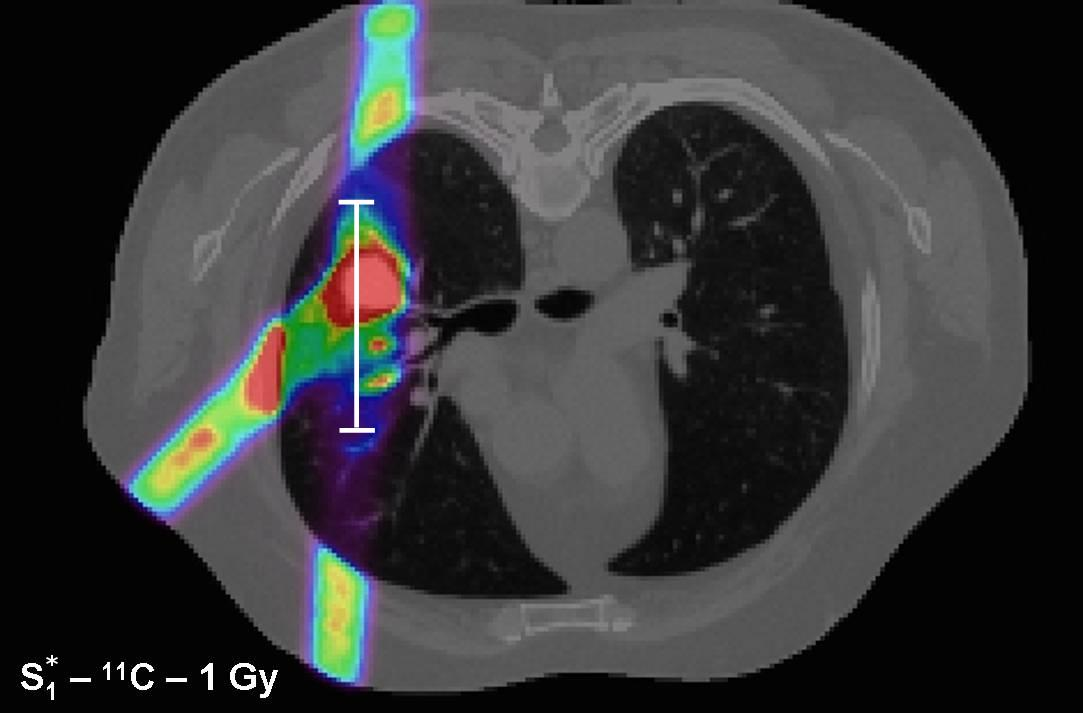
\includegraphics[width=6cm,height=40mm]{figures/gaussPET_C11_v2.jpg}
  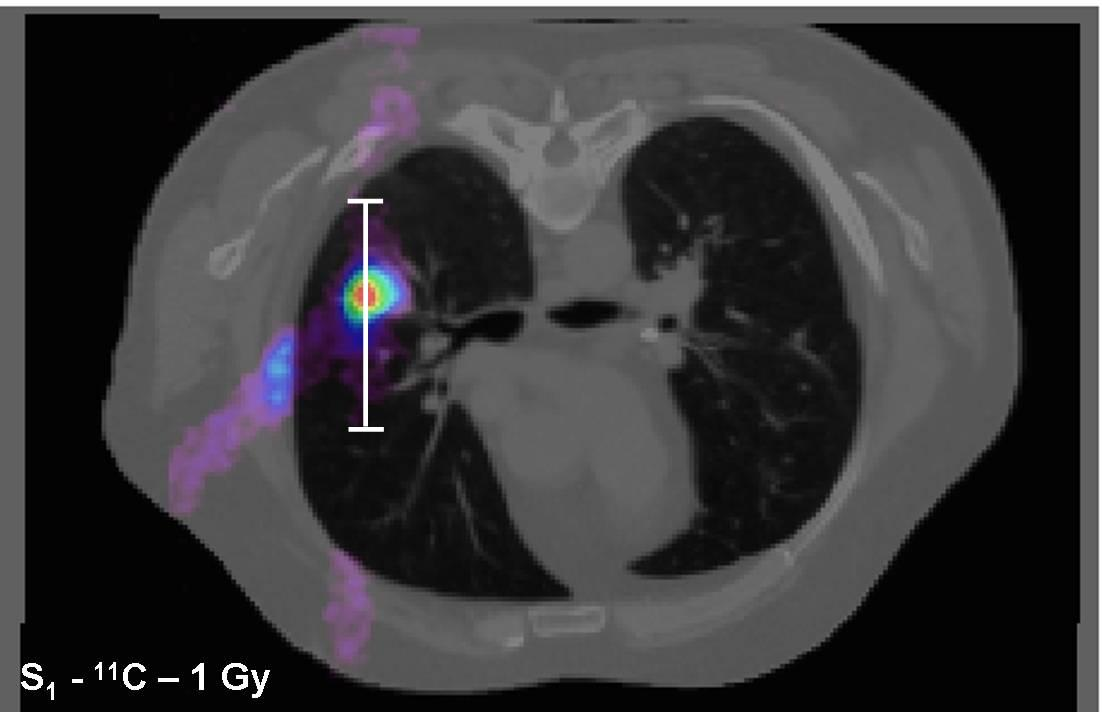
\includegraphics[width=6cm,height=40mm]{figures/C11_1Gy_v2.jpg}
  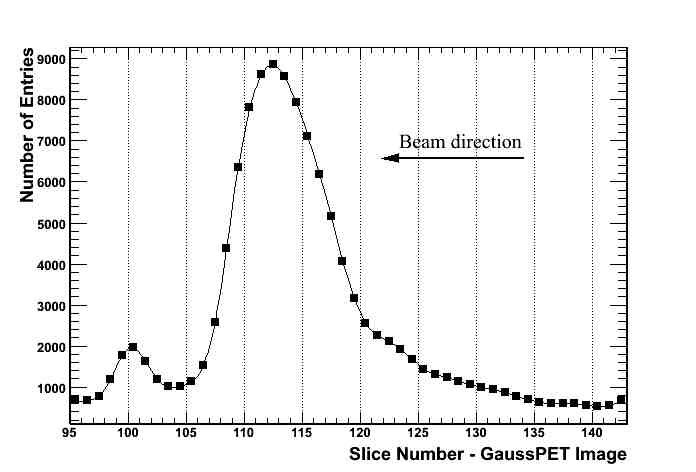
\includegraphics[width=65mm,height=45mm]{figures/prof_gaussPET_C11_v1.jpg}
  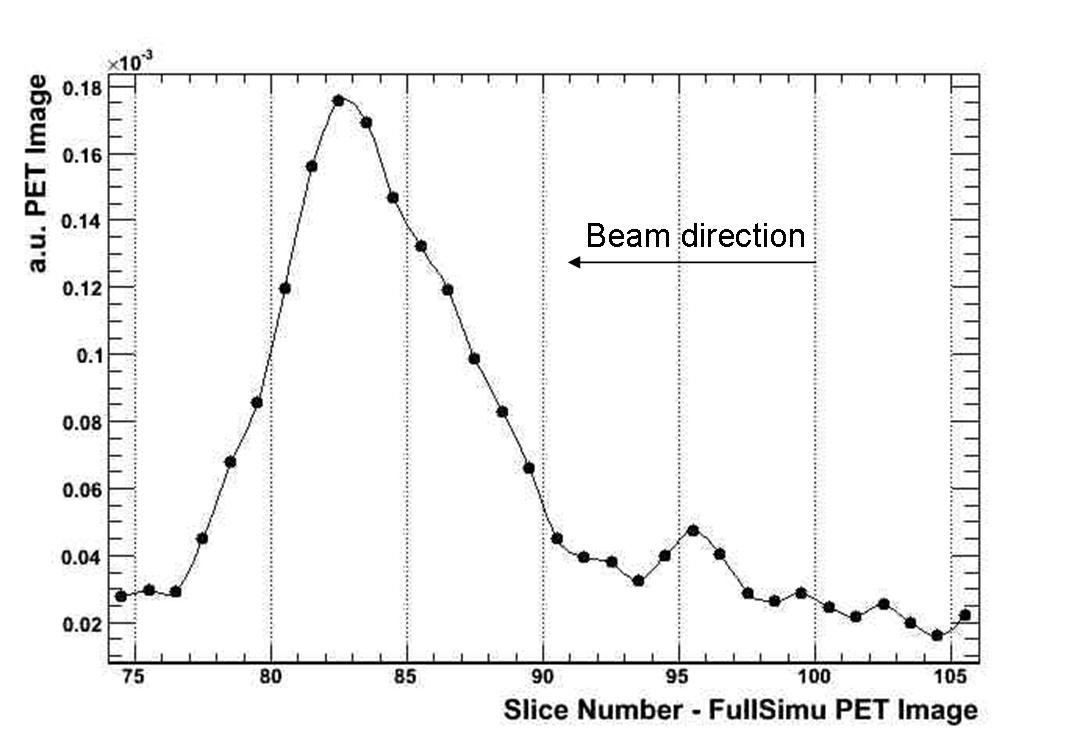
\includegraphics[width=65mm,height=45mm]{figures/1GyFullPET_v1.jpg}
  \caption{Comparison between configurations $S_{1}^{*}$ and
    $S_{1}$. It illustrates the differences between the PET images
    obtained with Gaussian smoothing (left) with the ones obtained
    with a complete PET system simulated by Monte-Carlo.}
  \label{fig:fig3}
\end{figure}

\dsnote{Les images sont très différentes en terme de représentation
  couleurs ! Comment as tu normalisé les échelles ? Il faut l'indiquer
  dans le texte je crois.}

\begin{table}[htbp]
  \begin{center}
    \begin{tabular}{|c|c|c|} \hline
      Configurations                & $L$ (mm)          & Peak position (mm)    \\\hline
%      &  mm                  & mm                       \\ \hline \hline
      $S_{1}$  (full PET)                     & 6.5                  &  119.2            \\ \hline 
      $S_{1}^{*}$  (Gaussian PET)                 & 8                    &  117.8         \\ \hline 
      $\Delta_{L}(S_{1}^{*};S_{1})$         &         \multicolumn{2}{c|}{18.7 $\%$}    \\ \hline\hline
    \end{tabular}
  \end{center} 
  \caption{\it Quantitative differences between Gaussian-based PET modelling
    and full system simulation.}
  \label{tab:gauss}
\end{table}

We also studied the contribution of $^{15}$O isotope to the final PET
images by comparing configurations $S_{3}^{*}$ and $S_{3}$. The
differences between the two PET images are illustrated by the
figure~\ref{fig:fig4}. They were around around 1.1\%, as
quantitatively presented in table~\ref{tab:O15}. Indeed, it is known
that $^{11}$C production is higher than $^{15}$O production by a
factor 4-5 and that the half-life is 2 minutes for $^{15}$O and 20
minutes for $^{11}$C. It is thus not necessary at this level of
knowledge to develop a dedicated method to correct the $^{11}$C PET
image from the $^{15}$O contribution.

\begin{figure}[!htbp]
  \begin{center}
    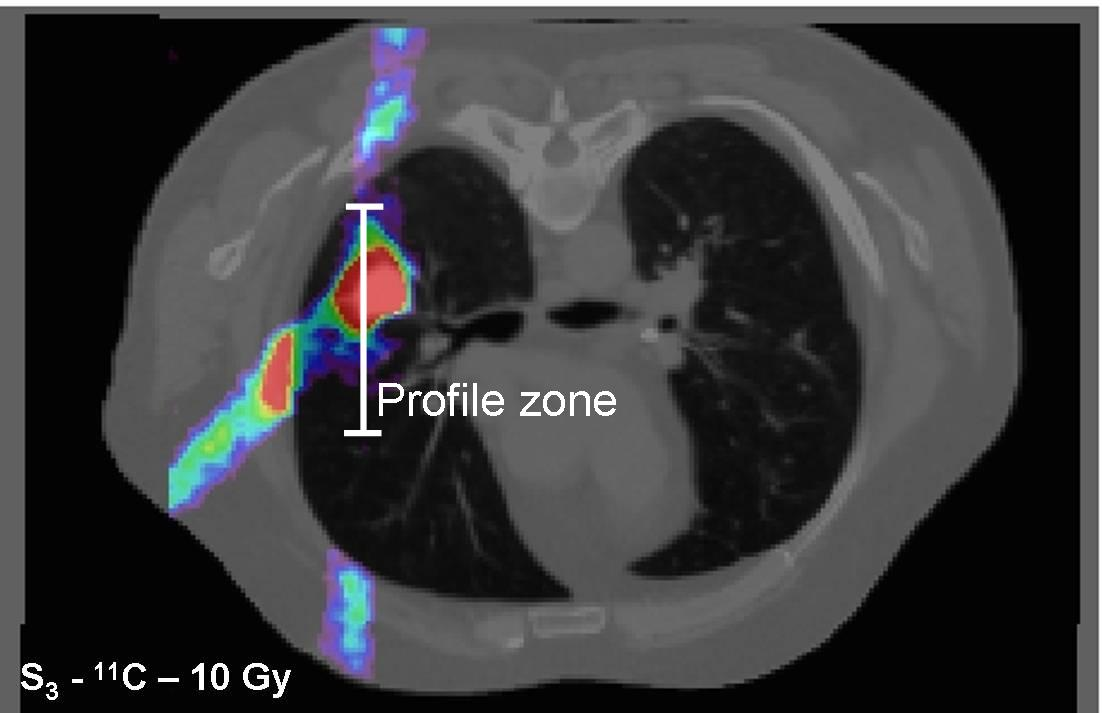
\includegraphics[width=6cm,height=40mm]{figures/C11_10Gy_v2.jpg}   
    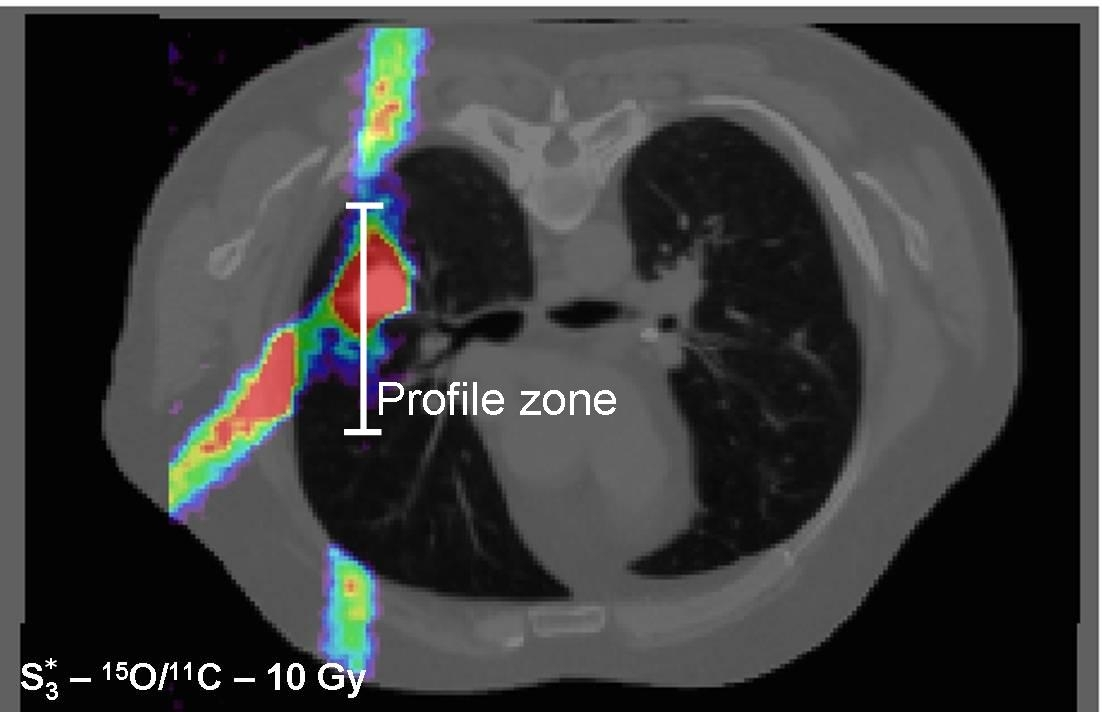
\includegraphics[width=60mm,height=40mm]{figures/C11_O15_10Gy_v2.jpg}
    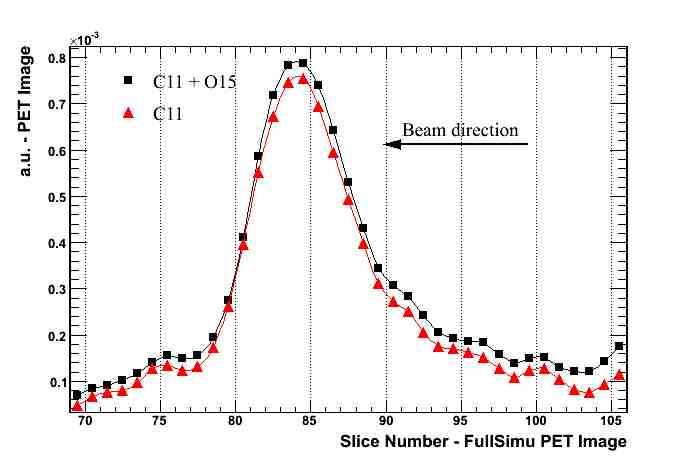
\includegraphics[width=75mm,height=50mm]{figures/prof_C11_O15_10Gy_v3.jpg}
    \caption{Comparison between configurations $S_{3}$ and $S_{3}^{*}$
      to illustration the influence of the $^{15}$O isotope on the PET
      image. The image at left was obtained by considering $^{11}$C
      only, and the image at right with both $^{11}$C and $^{15}$O.}
  \end{center}
  \label{fig:fig4}
\end{figure}

\begin{table}[htbp]
\begin{center}
\begin{tabular}{|c|c|c|} \hline
 Configurations                & $L$ (mm)            & Max peak
 position (mm)       \\\hline
%                              &  mm                  & mm                       \\ \hline \hline
$S_{3}$  ($^{11}$C only)                   & 9.1                  &  116.6                       \\ \hline
$S_{3}^{*}$ ($^{11}$C and $^{15}$O)          & 9.2                  &  115.3               \\ \hline
$\Delta_{L}(S_{3}^{*};S_{3})$         &        \multicolumn{2}{c|}{1.1 $\%$}     \\ \hline\hline
\end{tabular}
\end{center} 
\caption{\it Difference between PET images obtained from $^{11}$C only
  and from both $^{11}$C and $^{15}$O.}
\label{tab:O15}
\end{table}


The last analysis concerns the influence of the dose to the PET image
quality (configurations $S_{1}$, $S_{2}$ and
$S_{3}$). Table~\ref{tab:dose} and figure~\ref{fig:fig5} show the high
sensitivity to the level of delivered dose. In particular, $L$ varies
from $6.5$ to $9.1$ mm (40\%). Care must thus be taken when distal
falloff are studied from PET images.

% \sjnote{Je dois completer a ce niveau dans l'explication}
% These results illustrate clearly the high correlation and sensitivity between the dose on the target and the capability to have a quantitative analysis with the control PET imaging.

\begin{figure}[!h]
  \begin{center}
  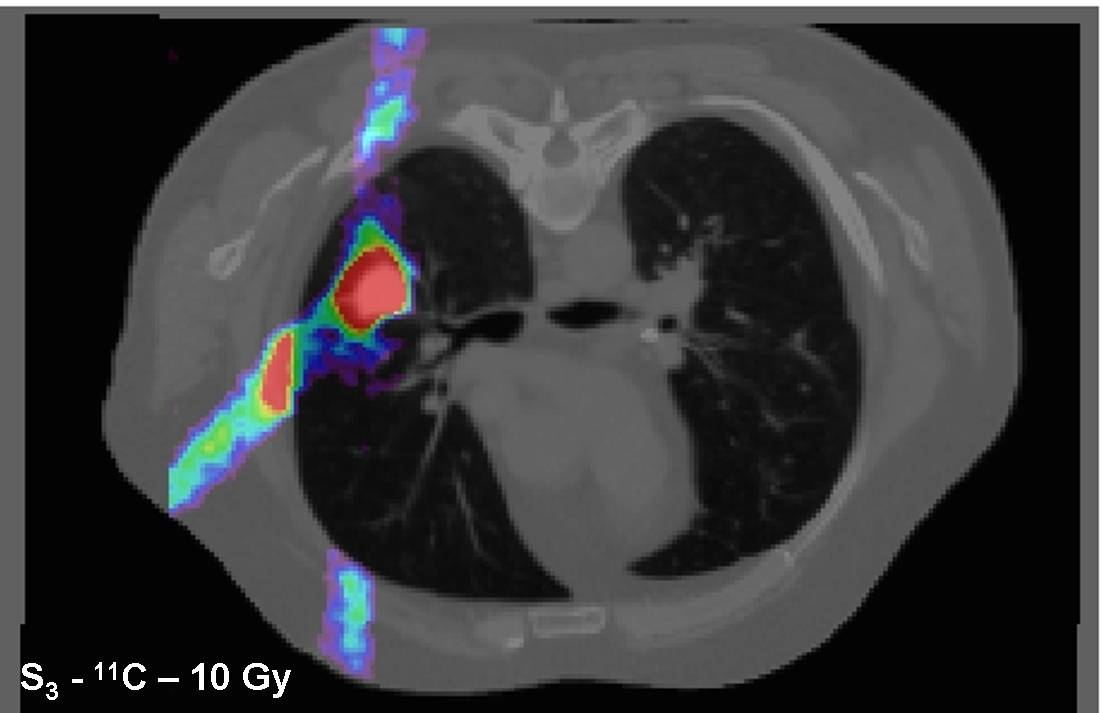
\includegraphics[width=6cm,height=40mm]{figures/C11_10Gy_v1.jpg}
  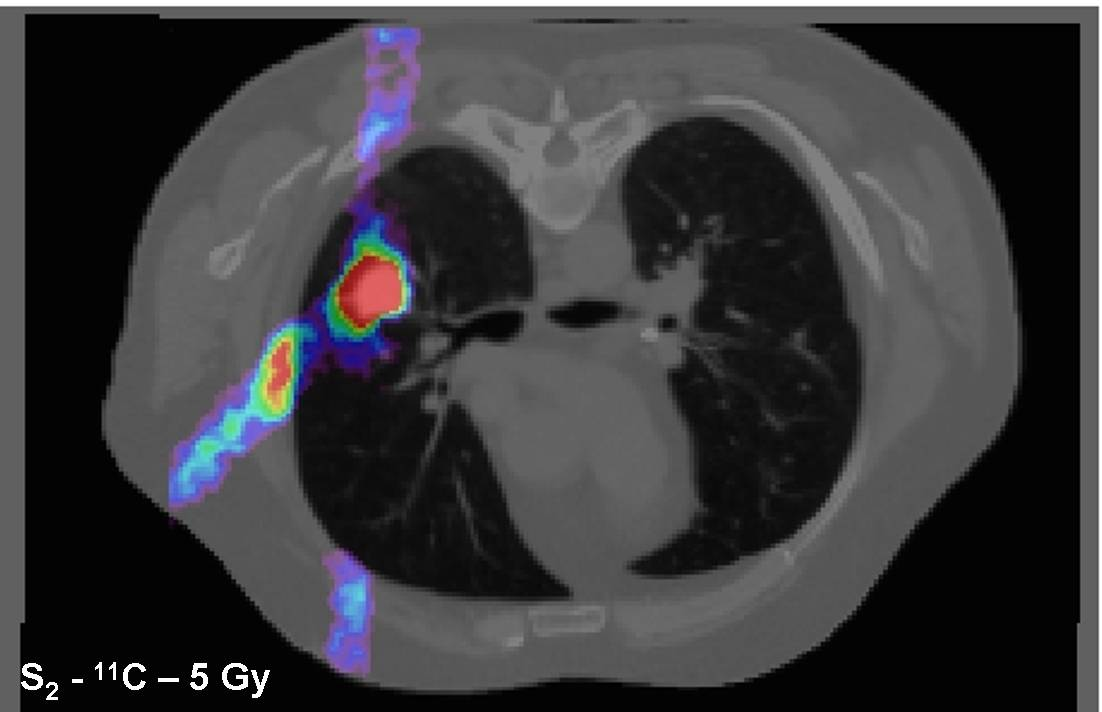
\includegraphics[width=6cm,height=40mm]{figures/C11_5Gy_v1.jpg}
  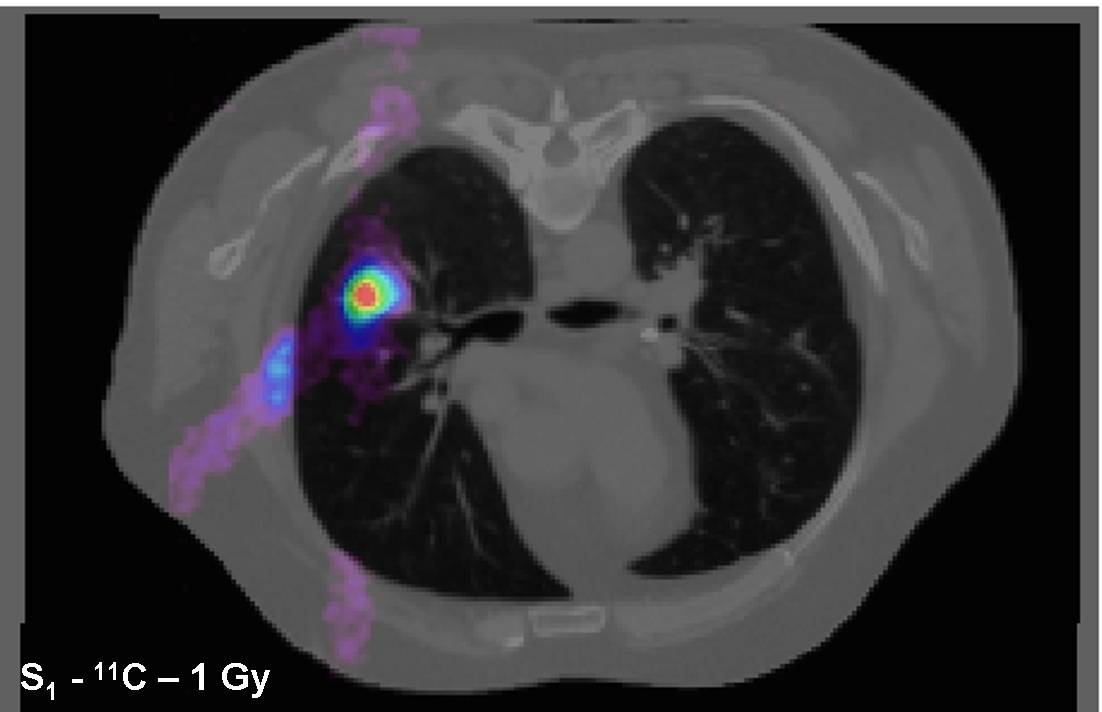
\includegraphics[width=6cm,height=40mm]{figures/C11_1Gy_v1.jpg}
  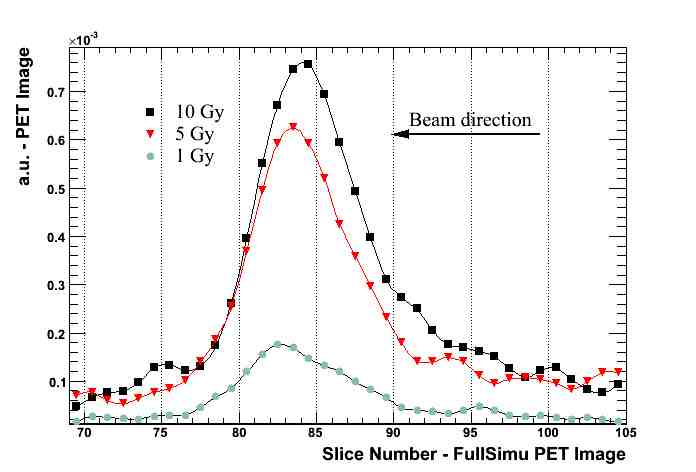
\includegraphics[width=75mm,height=55mm]{figures/10-5-1-Gy.jpg}
  \caption{Images obtained from the complete PET system simulations
    for 10, 5 and 1 Gy delivered to the tumor. \dsnote{manque
      l'endroit du profil sur la figure}}
  \end{center}
  \label{fig:fig5}
\end{figure}



\begin{table}[htbp]
\begin{center}
\begin{tabular}{|c|c|c|} \hline
 Configurations                & $L$ (mm)            & Max peak position (mm)      \\\hline
%                              &  mm                  & mm                       \\ \hline \hline
$S_{3}$                       & 9.1                  &  116.6                       \\ \hline
$S_{2}$                       & 7.8                  &  116.6                 \\ \hline
$S_{1}$                       & 6.5                  &  119.2            \\ \hline 
$\Delta_{L}(S_{3};S_{2})$         &       \multicolumn{2}{c|}{16.5 $\%$}  \\ \hline
$\Delta_{L}(S_{2};S_{1})$         &        \multicolumn{2}{c|}{20.0 $\%$} \\ \hline
$\Delta_{L}(S_{3};S_{1})$         &        \multicolumn{2}{c|}{40.0 $\%$}  \\ \hline \hline
\end{tabular}
\end{center} 
\caption{\it Quantitative estimators to evaluate the relation between the tumour deposited dose and the $^{11}$C PET image monitoring.}
\label{tab:dose}
\end{table}


\dsnote{On ajouterai pas une ligne de résultat sur les temps de calcul
  sur Titane ?}

%%%%%%%%%%%%%%%%%%%%%%%%%%%%%%%%%%%%%%%%%%%%%%%%%%%%%%%%%%%%%%%%%%%%%%%%%%%%%%%%%%%%%%%
\clearpage
\section{Conclusion}

This feasibility study illustrates the capability of GATE to perform
realistic simulations in the fields of hadrontherapy and nuclear
imaging. This work shows that, thanks to the high scalability of the
code, the GATE platform is a well suited tool to produce scientific
data from highly realistic simulations. It was illustrated with
simulations of a complete carbon beam cancer treatment plan on a
patient CT image, coupled with a full PET acquisition system used for
dose monitoring.

% This characteristic should be an advantage for the production
% of database to work on protocol optimization, or to define and
% validate analytical models for dose monitoring.

The simulations were used to show that the deposited dose should be
higher than 1 Gy in the target volume. We also show that it is not
necessary to develop an isotope deconvolution method to quantified the
correlation between $^{11}$C distribution and dose deposited by
$^{12}$C. We finally illustrate the importance of using a realistic
simulation of the PET system, instead of a Gaussian function response
as it is generally done. We showed that GATE is adapted to design
imaging systems for hadrontherapy, to optimize the sensitivity and the
quantitative performances for monitoring the beam delivery. When using
PET as a dose monitoring tool in hadrontherapy, a major challenge will
be the detection with a low number of events. The performances of the
imaging system and the image reconstruction algorithm are thus
crucial.

% It will be essential to validate all these new approaches to
% produce very realistic data sets of irradiation protocols associated
% to the imaging system for therapeutic control.

% As an example, some approaches focused on continuous
% space-time reconstruction 
% developments~\cite{Fall2011}. 
\dsnote{Que vient faire la ref sur le 4D ? on l'évoque pas ici, si ?
  Tu peux le citer plus tôt quand on évoque la reconstruction, non ?}


% According to the relative
% contribution of the different $\beta^+$ emitters for a
% post-irradiation PET acquisition longer that 10 minutes, we conclude
% that it is not necessary to develop some isotope deconvolution methods
% to quantified the correlation between $^{11}$C distribution and dose
% deposited by $^{12}$C.


%NEXT BIG POINT : TIME STRUCTURE OF THE BEAM + phase-space


%%%%%%%%%%%%%%%%%%%%%%%%%%%%%%%%%%%%%%%%%%%%%%%%%%%%%%%%%%%%%%%%%%%%%%%%%%%%%%%%%%%%%%%
%\bibliographystyle{jphysicsB}
%\bibliographystyle{agsm}
~\\\bibliographystyle{unsrt}
%\bibliographystyle{jmr}
%\bibliographystyle{agsm}

%\bibliographystyle{unsrt}
\bibliography{gc}
%%%%%%%%%%%%%%%%%%%%%%%%%%%%%%%%%%%%%%%%%%%%%%%%%%%%%%%%%%%%%%%%%%%%%%%%%%%%%%%%%%%%%%%
\end{document}
